% Options for packages loaded elsewhere
\PassOptionsToPackage{unicode}{hyperref}
\PassOptionsToPackage{hyphens}{url}
%
\documentclass[
  12pt,
  a4paper,
]{article}
\usepackage{amsmath,amssymb}
\usepackage{iftex}
\ifPDFTeX
  \usepackage[T1]{fontenc}
  \usepackage[utf8]{inputenc}
  \usepackage{textcomp} % provide euro and other symbols
\else % if luatex or xetex
  \usepackage{unicode-math} % this also loads fontspec
  \defaultfontfeatures{Scale=MatchLowercase}
  \defaultfontfeatures[\rmfamily]{Ligatures=TeX,Scale=1}
\fi
\usepackage{lmodern}
\ifPDFTeX\else
  % xetex/luatex font selection
\fi
% Use upquote if available, for straight quotes in verbatim environments
\IfFileExists{upquote.sty}{\usepackage{upquote}}{}
\IfFileExists{microtype.sty}{% use microtype if available
  \usepackage[]{microtype}
  \UseMicrotypeSet[protrusion]{basicmath} % disable protrusion for tt fonts
}{}
\makeatletter
\@ifundefined{KOMAClassName}{% if non-KOMA class
  \IfFileExists{parskip.sty}{%
    \usepackage{parskip}
  }{% else
    \setlength{\parindent}{0pt}
    \setlength{\parskip}{6pt plus 2pt minus 1pt}}
}{% if KOMA class
  \KOMAoptions{parskip=half}}
\makeatother
\usepackage{xcolor}
\usepackage[top=30mm,left=30mm,right=20mm,bottom=20mm]{geometry}
\usepackage{graphicx}
\makeatletter
\def\maxwidth{\ifdim\Gin@nat@width>\linewidth\linewidth\else\Gin@nat@width\fi}
\def\maxheight{\ifdim\Gin@nat@height>\textheight\textheight\else\Gin@nat@height\fi}
\makeatother
% Scale images if necessary, so that they will not overflow the page
% margins by default, and it is still possible to overwrite the defaults
% using explicit options in \includegraphics[width, height, ...]{}
\setkeys{Gin}{width=\maxwidth,height=\maxheight,keepaspectratio}
% Set default figure placement to htbp
\makeatletter
\def\fps@figure{htbp}
\makeatother
\setlength{\emergencystretch}{3em} % prevent overfull lines
\providecommand{\tightlist}{%
  \setlength{\itemsep}{0pt}\setlength{\parskip}{0pt}}
\setcounter{secnumdepth}{5}
\ifLuaTeX
\usepackage[bidi=basic]{babel}
\else
\usepackage[bidi=default]{babel}
\fi
\babelprovide[main,import]{brazilian}
% get rid of language-specific shorthands (see #6817):
\let\LanguageShortHands\languageshorthands
\def\languageshorthands#1{}
\usepackage{longtable}
\LTcapwidth=.95\textwidth
\linespread{1.15}
\usepackage{hyperref}
\usepackage{array}
\usepackage{caption}
\usepackage{graphicx}
\usepackage{siunitx}
\usepackage{multirow}
\usepackage{hhline}
\usepackage{calc}
\usepackage{tabularx}
\usepackage{fontawesome}
\usepackage[para,online,flushleft]{threeparttable}
\usepackage{placeins}
\usepackage{booktabs}
\usepackage{longtable}
\usepackage{array}
\usepackage{multirow}
\usepackage{wrapfig}
\usepackage{float}
\usepackage{colortbl}
\usepackage{pdflscape}
\usepackage{tabu}
\usepackage{threeparttable}
\usepackage{threeparttablex}
\usepackage[normalem]{ulem}
\usepackage{makecell}
\usepackage{xcolor}
\ifLuaTeX
  \usepackage{selnolig}  % disable illegal ligatures
\fi
\usepackage[]{natbib}
\bibliographystyle{plainnat}
\IfFileExists{bookmark.sty}{\usepackage{bookmark}}{\usepackage{hyperref}}
\IfFileExists{xurl.sty}{\usepackage{xurl}}{} % add URL line breaks if available
\urlstyle{same}
\hypersetup{
  pdftitle={Relatório Econômico-Social da Cidade de Aracaju},
  pdfauthor={José Wilas Alves de Farias},
  pdflang={pt-BR},
  pdfkeywords={PNADcT, Desemprego, Renda, Aracaju},
  hidelinks,
  pdfcreator={LaTeX via pandoc}}

\title{Relatório Econômico-Social da Cidade de Aracaju}
\author{José Wilas Alves de Farias}
\date{02 setembro, 2023}

\begin{document}
\maketitle
\begin{abstract}
Este trabalho se trata de um pequeno relatório de autoria própria e sem
pretenções de publicação de artigo. Nele será trabalhado dados da PNADcT
em diversos pontos importantes do mercado de trabalho da Cidade de
Aracaju, Capital do Estado de Sergipe, englobando desemprego, renda
média, escolaridade e setores produtivos.
\end{abstract}

\hypertarget{introduuxe7uxe3o}{%
\section{Introdução}\label{introduuxe7uxe3o}}

Este trabalho é desenvolvido apenas como uma forma de pensar o município
de forma crítica e análitica de forma não detalhada, mas observando
pontos importantes da situação econômica e social da capital do estado
de Sergipe.

O trabalho está dividido em seis capítulos além dessa introdução. O
segundo capítulo analisa a População Total do Município por Gênero e a
Renda Média. O terceito capítulo trata da População na Força de
Trabalho, Ocupadas e Desocupadas, Fora da Força de Trabalho e
Desalentados. O quarto capítulo estuda a População NEM-NEM por Nível de
Instrução. O quinto capítulo estuda os Jovens Desocupados por Nível de
Instrução. E, o sexto capítulo analisa as Pessoas Ocupadas por Setor
Produtivo.

\hypertarget{total-da-populauxe7uxe3o-de-aracaju-por-sexo} da população da capital do estado de Sergipe é formada por
mulheres. Mostra-se crescimento apróximado entre os trimestres
analisados, e com trajetória crescente da população de Aracaju, com
redução do quantitativo de homens no 2º trimestre de 2022 e 1º trimestre
de 2023.

\begingroup\fontsize{9}{11}\selectfont

\begin{longtable}[t]{ccccr}
\caption{\label{tab:tab1}\label{tab1}Total da População por Sexo em Aracaju e Renda Média, 
2022.1 a 2023.1}\\
\toprule
Trimestre & Homem & Mulher & Total & Renda Média\\
\midrule
2022.1 & 324.816 & 352.435 & 677.251 & 3.108,09\\
\cellcolor[HTML]{DCDCDC}{2022.2} & \cellcolor[HTML]{DCDCDC}{319.497} & \cellcolor[HTML]{DCDCDC}{359.615} & \cellcolor[HTML]{DCDCDC}{679.112} & \cellcolor[HTML]{DCDCDC}{3.136,40}\\
2022.3 & 321.940 & 359.022 & 680.962 & 3.084,29\\
\cellcolor[HTML]{DCDCDC}{2022.4} & \cellcolor[HTML]{DCDCDC}{325.904} & \cellcolor[HTML]{DCDCDC}{356.896} & \cellcolor[HTML]{DCDCDC}{682.800} & \cellcolor[HTML]{DCDCDC}{3.521,83}\\
2023.1 & 323.962 & 360.664 & 684.626 & 3.865,34\\
\bottomrule
\multicolumn{5}{l}{\rule{0pt}{1em}\textit{Fonte: IBGE (2023).}}\\
\multicolumn{5}{l}{\rule{0pt}{1em}}\\
\end{longtable}
\endgroup{}

Já no caso das mulheres ocorreu redução no 3º e de forma mais relevante
no 4º trimestre de 2022. Olhando a trajetória da renda, tem-se que
ocorreu redução no 3º trimestre de 2022, mas que retornou a sua
tendência de crescimento no trimestre seguinte, chegando a
\texttt{13,3\%} de diferênça entre o 4º e o 1º trimestre de 2022, e
aumento de \texttt{24,4\%} entre o primerio trimestre de 2022 até o
primeiro trimestre de 2023, com renda média de R\$ 3.865,34.

\FloatBarrier
\begin{figure}

{\centering 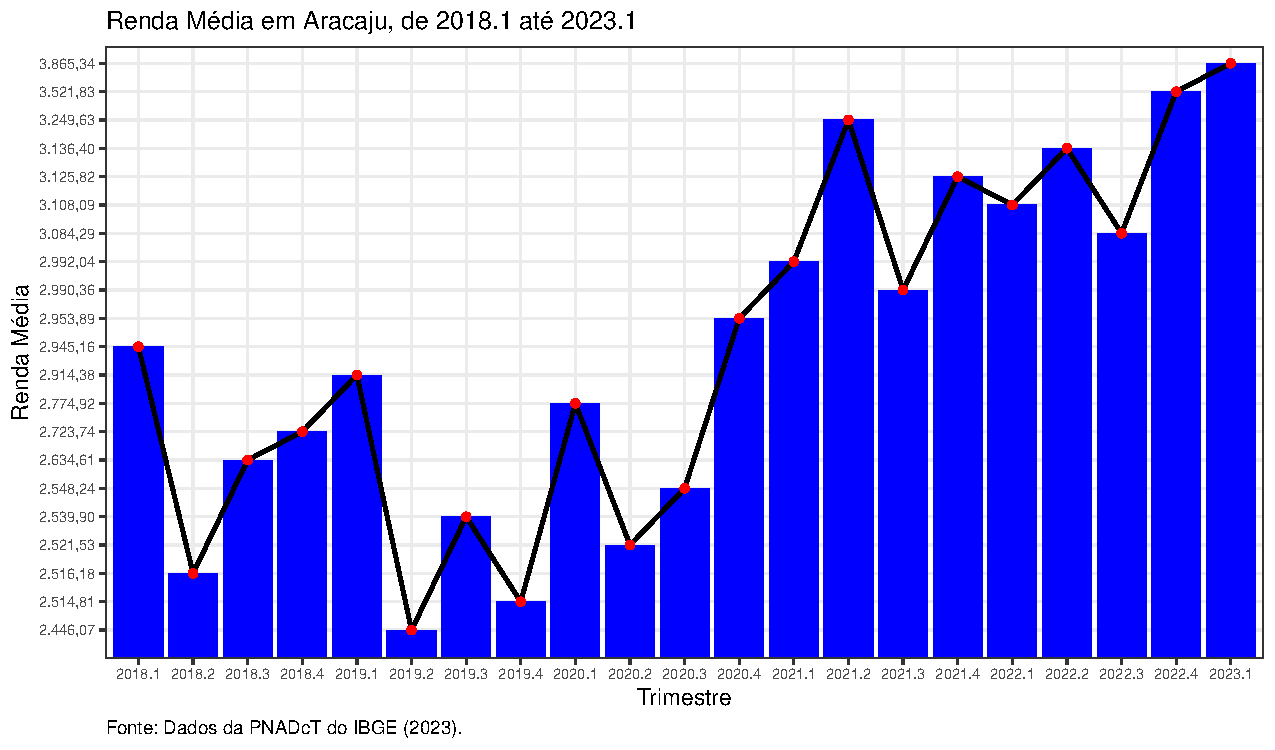
\includegraphics[width=1\linewidth]{wilas_relatorio_files/figure-latex/fig1-1} 

}

\caption{Renda Média em Aracaju, de 2018.1 até 2023.1}\label{fig:fig1}
\end{figure}
\FloatBarrier

A Figura \ref{fig:fig1} mostra a renda média da cidade de Aracaju do
período do 1º trimestre de 2018 até o 1º trimestre de 2023. Nele é
possível análisar o período de forma clara, e pode-se perceber que do 2º
trimestre de 2018 até 3º trimestre de 2020 a renda média foi inferior ao
primeiro trimestre de 2018, mostrando que em todo esse peíodo não se
demostrou sinais de melhoras no poder aquisitivo na capital do estado de
Sergipe.

A melhora só se iniciou apartir do 4º trimestre de 2020, chegando ao
ápice em dois trimestre e volta a cair a partir de então e apenas
apresenta melhora no 4º trimestre de 2022. Isso mostra correlação com a
administração federal, em que no primeiro um ano e nove meses no poder
do então presidente da república a cidade de Aracaju não mostrou sinais
de melhora em sua renda média.

A melhora veio a ser visualizada a partir do último trimestre de 2020,
fruto da espectativa do recebimento do auxílio emergencial proveniente
do governo federal, e sem outros projetos de melhorias na renda média a
contínua e crescente melhoria estava atrelada apenas a esse único
projeto, em sua manutenção e no aumento do número de beneficiários que
necessitavam dessa fonte de recurso para sua sobrevivência e de seus
familiares.

Com o bum da melhoria no poder aquisitivo, que durou apenas dois
trimestres, chegando a seu ápice logo no segundo trimestre de 2021 e não
houve até o fim do então governo federal outro mês que apresentase renda
média superior a esse trimestre. Nesse sentido, mostra que o recebimento
apenas manteve o valor da renda e não repercurtiu essa espectativa em
outros indicadores econômicos.

\hypertarget{populauxe7uxe3o-na-foruxe7a-de-trabalho-fora-da-foruxe7a-de-trabalho-ocupada-desocupada-e-em-desalento-em-aracaju}{%
\section{População na Força de Trabalho, Fora da Força de Trabalho,
Ocupada, Desocupada e em Desalento em
Aracaju}\label{populauxe7uxe3o-na-foruxe7a-de-trabalho-fora-da-foruxe7a-de-trabalho-ocupada-desocupada-e-em-desalento-em-aracaju}}

De início a Tabela \ref{tab2} mostra que há cresciemtno da população da
capital do estado, mas em comparação com a Tabela \ref{tab1} demonstra
que esse aumento representa pessoas em idade não ativa. Destaca-se a
grande queda das Pessoas na Força do Trabalho, coupadas e desocupadas,
em comparação das Pessoas Fora da força de trabalho.

\begingroup\fontsize{9}{11}\selectfont

\begin{longtable}[t]{>{\centering\arraybackslash}p{1cm}>{\centering\arraybackslash}p{3.2cm}>{\centering\arraybackslash}p{3.2cm}>{\centering\arraybackslash}p{2cm}>{\centering\arraybackslash}p{2cm}>{\centering\arraybackslash}p{2cm}}
\caption{\label{tab:tab2}\label{tab2}População na Força de Trabalho, Fora da Força de Trabalho, Ocupada, Desocupada e em Desalento em Aracaju, 2022.1 a 2023.1}\\
\toprule
Trimestre & Pessoas na força de trabalho & Pessoas fora da força de trabalho & Pessoas ocupadas & Pessoas desocupadas & Pessoas desalentadas\\
\midrule
2022.1 & 367.705 & 195.409 & 314.462 & 53.243 & 11.994\\
\cellcolor[HTML]{DCDCDC}{2022.2} & \cellcolor[HTML]{DCDCDC}{362.663} & \cellcolor[HTML]{DCDCDC}{197.780} & \cellcolor[HTML]{DCDCDC}{314.610} & \cellcolor[HTML]{DCDCDC}{48.052} & \cellcolor[HTML]{DCDCDC}{14.807}\\
2022.3 & 356.474 & 201.020 & 309.245 & 47.229 & 15.927\\
\cellcolor[HTML]{DCDCDC}{2022.4} & \cellcolor[HTML]{DCDCDC}{356.726} & \cellcolor[HTML]{DCDCDC}{198.548} & \cellcolor[HTML]{DCDCDC}{310.155} & \cellcolor[HTML]{DCDCDC}{46.571} & \cellcolor[HTML]{DCDCDC}{10.245}\\
2023.1 & 344.165 & 218.839 & 301.091 & 43.073 & 11.671\\
\bottomrule
\multicolumn{6}{l}{\rule{0pt}{1em}\textit{Fonte: IBGE (2023).}}\\
\multicolumn{6}{l}{\rule{0pt}{1em}}\\
\end{longtable}
\endgroup{}

Para o primeiro grande grupo, PEA, tem-se que o impacto da redução
recaiu em grande parte no número de pessoas ocupadas, que saiu de
314.462 pessoas ocupadas para 301.091 pessoas, 1º trimestre de 2022 e
2023, respectivamente. Por outro lado o número de desempregados caiu de
53.243 (Taxa de Desemprego de 14.5\%, Tabela \ref{tab13}) para 43.073
(Taxa de Desemprego de 12.5\%, Tabela \ref{tab13}) pessoas, uma queda de
aproximadamente \emph{10.170} pessoas, 1º trimestre de 2022 a 2023
respectivamente, queda inferior as de aproximadamente \emph{13.371}
pessoas das pessoas ocupadas.

\begingroup\fontsize{9}{11}\selectfont

\begin{longtable}[t]{ccc}
\caption{\label{tab:tab13}\label{tab13}Taxa de Ocupação e Desocupação na Capital, 2022.4 a 2023.1}\\
\toprule
Trimestres & Taxa de Desocupação & Taxa de Ocupação\\
\midrule
2022.1 & 14,5 & 85,5\\
\cellcolor[HTML]{DCDCDC}{2022.2} & \cellcolor[HTML]{DCDCDC}{13,2} & \cellcolor[HTML]{DCDCDC}{86,8}\\
2022.3 & 13,2 & 86,8\\
\cellcolor[HTML]{DCDCDC}{2022.4} & \cellcolor[HTML]{DCDCDC}{13,1} & \cellcolor[HTML]{DCDCDC}{86,9}\\
2023.1 & 12,5 & 87,5\\
\bottomrule
\multicolumn{3}{l}{\rule{0pt}{1em}\textit{Fonte: IBGE (2023).}}\\
\multicolumn{3}{l}{\rule{0pt}{1em}}\\
\end{longtable}
\endgroup{}

É importante salientar que a há uma tragetória de queda do número de
pessoas desocupados, mas se apresenta não de forma consistênte e que é
de extrema importância dado que a taxa de desemprego ainda estava em
13.1\% no 4º trimestre de 2022 e no 1º Trimestre de 2023 está em 12.5\%.
A redução apresentada no número de pessoas desocupadas em termos
absolutos, não representou melhora no quadro empregatício do município,
o que pode supor é que essa massa de desempregados transferiu-se para o
número de Pessoas Fora da Força de Trabalho e um pequeno número foi para
os desalentados, entendimento corroborado pelo aumento desses dois
indicadores.

Olhando para as pessoas em desalento, as quais representam uma parte as
PÑEA, que chegou ao auge nos 2º e 3º trimestre de 2022, chegando as
15.927 pessoas que devido a não conseguirem ocupação por um longo
período de tempo pararam de procurar emprego. Apesar da redução do
número de desalentados, ainda não se mostraram efetivas e eficientes as
medidas tomadas para mitigar essa triste realidade que está a si
transformar em ``patologia'' na capital do estado.

\begingroup\fontsize{9}{11}\selectfont

\begin{longtable}[t]{ccc}
\caption{\label{tab:tab3}\label{tab3}Pessoas que Estudam em Aracaju, 2022.1 a 2023.1}\\
\toprule
Trimestres & Estudam & Não Estudam\\
\midrule
2022.1 & 181.670 & 453.715\\
\cellcolor[HTML]{DCDCDC}{2022.2} & \cellcolor[HTML]{DCDCDC}{180.855} & \cellcolor[HTML]{DCDCDC}{460.077}\\
2022.3 & 177.661 & 465.271\\
\cellcolor[HTML]{DCDCDC}{2022.4} & \cellcolor[HTML]{DCDCDC}{187.619} & \cellcolor[HTML]{DCDCDC}{451.997}\\
2023.1 & 176.399 & 459.864\\
\bottomrule
\multicolumn{3}{l}{\rule{0pt}{1em}\textit{Fonte: IBGE (2023).}}\\
\multicolumn{3}{l}{\rule{0pt}{1em}}\\
\end{longtable}
\endgroup{}

Na Tabela \ref{tab3} há uma tendência de aumento do número de pessoas
que não estudam em Aracaju, apesar do aumento/retomada das pessoas a
estudar no 4º trimestre de 2022, mas já no 1º trimestre de 2023 há o
aumento do número de pessoas que não estudam em torno \emph{7.867}
(\texttt{1,7\%}) do total de \ensuremath{4.5986407\times 10^{5}} pessoas
(\texttt{72\%} da População Total).

Na Tabela \ref{tab4}, tem-se que algumas pessoas podem entender como
possitivo, mas que de fato é algo preocupante. Em que no último
trimestre de 2022 houve aumento relevante do númnero de pessoas
desempregadas e que estudavam, mas no primeiro trimestre de 2023 esse
número voltou a cair, tendo uma leve sensação de melhora. Entretanto, é
de suma importância salientar que essa redução não refletiu no aumento
do número de pessoas empregadas, mas de aumento do número de pessoas que
além de estarem fora do mercado de trabalho pioram sua situação ao
deixarem de estudar e adquirirem novas competéncias.

\begingroup\fontsize{9}{11}\selectfont

\begin{longtable}[t]{>{\centering\arraybackslash}p{1cm}>{\centering\arraybackslash}p{3.2cm}>{\centering\arraybackslash}p{3.2cm}>{\centering\arraybackslash}p{3.2cm}>{\centering\arraybackslash}p{3.2cm}}
\caption{\label{tab:tab4}\label{tab4}Pessoas Ocupadas e Desocupadas que Estudam e Não Estudam em Aracaju, 2022.4 a 2023.1}\\
\toprule
Trimestre & Ocupadas Estudam & Ocupadas Não Estudam & Desocupadas Estudam & Desocupadas Não Estudam\\
\midrule
2022.1 & 39.251 & 275.210 & 12.621 & 40.623\\
\cellcolor[HTML]{DCDCDC}{2022.2} & \cellcolor[HTML]{DCDCDC}{37.896} & \cellcolor[HTML]{DCDCDC}{276.715} & \cellcolor[HTML]{DCDCDC}{13.696} & \cellcolor[HTML]{DCDCDC}{34.356}\\
2022.3 & 35.399 & 273.846 & 9.964 & 37.265\\
\cellcolor[HTML]{DCDCDC}{2022.4} & \cellcolor[HTML]{DCDCDC}{40.963} & \cellcolor[HTML]{DCDCDC}{269.193} & \cellcolor[HTML]{DCDCDC}{12.670} & \cellcolor[HTML]{DCDCDC}{33.901}\\
2023.1 & 38.408 & 262.683 & 8.766 & 34.307\\
\bottomrule
\multicolumn{5}{l}{\rule{0pt}{1em}\textit{Fonte: IBGE (2023).}}\\
\multicolumn{5}{l}{\rule{0pt}{1em}}\\
\end{longtable}
\endgroup{}

Como mostra a Tabela \ref{tab5}, População por Nivel de Instrução, há
redução do número de pessoas sem o curso fundamental completo, mas ainda
é preocupante essa situação levando em consideração que no 1º Trimestre
de 2023 cerca de \texttt{30\%} das pessoas ainda não concluíram o ensino
fundamental. Nesse sentido, mostra que houve redução de pessoas com
curso médio completo e acima, e podemos entender que há fuga de mentes
na capital do estado.

\begingroup\fontsize{9}{11}\selectfont

\begin{longtable}[t]{>{\raggedright\arraybackslash}p{7cm}cc}
\caption{\label{tab:tab5}\label{tab5}População por Nivel de Instrução em Aracaju, 2022.4 a 2023.1}\\
\toprule
Nivel & 2022.4 & 2023.1\\
\midrule
Sem instrução e menos de 1 ano de estudo & 31.559 & 29.817\\
\cellcolor[HTML]{DCDCDC}{Fundamental incompleto ou equivalente} & \cellcolor[HTML]{DCDCDC}{179.191} & \cellcolor[HTML]{DCDCDC}{163.326}\\
Fundamental completo ou equivalente & 31.054 & 46.958\\
\cellcolor[HTML]{DCDCDC}{Médio incompleto ou equivalente} & \cellcolor[HTML]{DCDCDC}{40.117} & \cellcolor[HTML]{DCDCDC}{42.550}\\
Médio completo ou equivalente & 166.959 & 165.382\\
\addlinespace
\cellcolor[HTML]{DCDCDC}{Superior incompleto ou equivalente} & \cellcolor[HTML]{DCDCDC}{46.322} & \cellcolor[HTML]{DCDCDC}{45.517}\\
Superior completo & 144.415 & 142.712\\
\bottomrule
\multicolumn{3}{l}{\rule{0pt}{1em}\textit{Fonte: IBGE (2023).}}\\
\multicolumn{3}{l}{\rule{0pt}{1em}}\\
\end{longtable}
\endgroup{}

Na Tabela \ref{tab6}, Nivel de Instrução das Pessoas que Não Estudam,
foi constatado que no 4º Trimestre de 2022 cerca de \texttt{71\%} da
população por nível de Instrução já deixaram de estudar e no 1º
Trimestre de 2023 ocorre aumento desse percentual para \texttt{72\%}
(\emph{459.864} pessoas). Há aumento do número de pessoas com o nível
fundamental completo, o que mostra uma melhora nesse nível no sentido
que parte das pessoas que estavam com fundamental incompleto conseguiram
concluir esse nível. Parcela dos alunos que estavam estudando o ensino
médio deram continuidade em seus estudos. Mas é importante destacar que
os alunos que já estavam no ensino médio não concluíram seus estudos e
isso ocorre para os demais níveis acima deste, o que caracteriza
abandono dos estudos ou até a saída desses jovens do município, fatos
que serão analisados posteriormente.

\begingroup\fontsize{9}{11}\selectfont

\begin{longtable}[t]{>{\raggedright\arraybackslash}p{7cm}cc}
\caption{\label{tab:tab6}\label{tab6}Nivel de Instrução das Pessoas que Não Estudam em Aracaju, 2022.4 a 2023.1}\\
\toprule
Nivel & 2022.4 & 2023.1\\
\midrule
Sem instrução e menos de 1 ano de estudo & 11.798 & 12.974\\
\cellcolor[HTML]{DCDCDC}{Fundamental incompleto ou equivalente} & \cellcolor[HTML]{DCDCDC}{94.121} & \cellcolor[HTML]{DCDCDC}{92.719}\\
Fundamental completo ou equivalente & 22.090 & 31.777\\
\cellcolor[HTML]{DCDCDC}{Médio incompleto ou equivalente} & \cellcolor[HTML]{DCDCDC}{26.680} & \cellcolor[HTML]{DCDCDC}{26.442}\\
Médio completo ou equivalente & 154.250 & 156.897\\
\addlinespace
\cellcolor[HTML]{DCDCDC}{Superior incompleto ou equivalente} & \cellcolor[HTML]{DCDCDC}{19.829} & \cellcolor[HTML]{DCDCDC}{17.383}\\
Superior completo & 123.229 & 121.672\\
\bottomrule
\multicolumn{3}{l}{\rule{0pt}{1em}\textit{Fonte: IBGE (2023).}}\\
\multicolumn{3}{l}{\rule{0pt}{1em}}\\
\end{longtable}
\endgroup{}

Logo, se observa a fuga de mentes ao observar redução do número de
pessoas por escolaridade com escolaridade acima do ensino médio, sendo
corroborado pela redução nesssas faixas das pessoas que deixaram de
estudar.

\hypertarget{populauxe7uxe3o-que-nuxe3o-estuda-e-nuxe3o-trabalha-nem-nem-por-nivel-de-instruuxe7uxe3o-em-aracaju}{%
\section{População que Não Estuda e Não Trabalha (Nem-Nem) por Nivel de
Instrução em
Aracaju}\label{populauxe7uxe3o-que-nuxe3o-estuda-e-nuxe3o-trabalha-nem-nem-por-nivel-de-instruuxe7uxe3o-em-aracaju}}

Tabela \ref{tab7} observa as pessoas desempregadas que deixara de
estudar, os Nem-Nem. tem-se que essa situação acontece em maior força
nas pessoas com baixa escolaridade com até ensino médio completo e
principalmente em pessoas com fundamental incompleto. Para essas faixas
houve aumento das pessoas Nem-Nem, em especial para as pessoas com
ensino fundamental incompleto que saiu de 5.301 para 8.316 pessoas no 1º
Trimestre de 2023. Destaca-se o aumento para faixa de pessoas com Ensino
Médio Completo que saiu de 13.513 para 15.958 pessoas NEM-NEM. Para os
níveis mais elevados houve redução. No geral tem-se aumento de 405
pessoas Nem-Nem na Capital do estado, em destaque para os níveis mais
baixos de escolaridade, do 4º Trimestre de 2022 para o 1º Trimestre de
2023.

\begingroup\fontsize{9}{11}\selectfont

\begin{longtable}[t]{>{\raggedright\arraybackslash}p{7cm}cc}
\caption{\label{tab:tab7}\label{tab7}Nem Estudam e Nem Trabalham por Nivel de Instrução em Aracaju, 2022.4 a 2023.1}\\
\toprule
Nivel & 2022.4 & 2023.1\\
\midrule
Sem instrução e menos de 1 ano de estudo & 757 & 1.080\\
\cellcolor[HTML]{DCDCDC}{Fundamental incompleto ou equivalente} & \cellcolor[HTML]{DCDCDC}{5.301} & \cellcolor[HTML]{DCDCDC}{8.316}\\
Fundamental completo ou equivalente & 2.491 & 824\\
\cellcolor[HTML]{DCDCDC}{Médio incompleto ou equivalente} & \cellcolor[HTML]{DCDCDC}{4.625} & \cellcolor[HTML]{DCDCDC}{2.937}\\
Médio completo ou equivalente & 13.513 & 15.958\\
\addlinespace
\cellcolor[HTML]{DCDCDC}{Superior incompleto ou equivalente} & \cellcolor[HTML]{DCDCDC}{1.827} & \cellcolor[HTML]{DCDCDC}{1.794}\\
Superior completo & 5.387 & 3.397\\
\bottomrule
\multicolumn{3}{l}{\rule{0pt}{1em}\textit{Fonte: IBGE (2023).}}\\
\multicolumn{3}{l}{\rule{0pt}{1em}}\\
\end{longtable}
\endgroup{}

Na Tabela \ref{tab8} mostra que no 1º Trimestre de 2023 ocorre redução
do Número de jovens em Aracaju, saiu de \emph{115.733} para
\emph{99.249} jovens. A análise dos motivos dessa redução não são objeto
de estudo desse trabalho. É demonstrado também a situação empregatícia
dos jovens, segundo o IBGE \citeyearpar{ibge2023} os jovens são
divididos em faixa de 15 a 29 anos, nesse sentido foi demostrado redução
de jovens de 15 a 19 anos ocupados e desocupados para variação do último
trimestre de 2022 para para o 1º Trimestre de 2023, mas embora tenha
havido redução em âmbos temos que foi remetid oem menot impacto no
núemro de despcucpados, o que demostra em certo sentido uma piora
relativa no quadro econômico-social da capital.

\begingroup\fontsize{9}{11}\selectfont

\begin{longtable}[t]{cccccc}
\caption{\label{tab:tab8}\label{tab8}Ocupação e Desocupação por Faixa Etária em Aracaju, 2022.4 a 2023.1}\\
\toprule
Trimestre & Faixa & Pessoas ocupadas & Pessoas desocupadas & Total & Taxa de Desocupação\\
\midrule
2022.4 & 15 a 19 & 10.222 & 9.083 & 19.304 & 47,0\\
\cellcolor[HTML]{DCDCDC}{2022.4} & \cellcolor[HTML]{DCDCDC}{20 a 24} & \cellcolor[HTML]{DCDCDC}{32.571} & \cellcolor[HTML]{DCDCDC}{10.620} & \cellcolor[HTML]{DCDCDC}{43.191} & \cellcolor[HTML]{DCDCDC}{24,6}\\
2022.4 & 25 a 29 & 44.252 & 8.986 & 53.238 & 16,9\\
\cellcolor[HTML]{DCDCDC}{2023.1} & \cellcolor[HTML]{DCDCDC}{15 a 19} & \cellcolor[HTML]{DCDCDC}{7.938} & \cellcolor[HTML]{DCDCDC}{7.273} & \cellcolor[HTML]{DCDCDC}{15.211} & \cellcolor[HTML]{DCDCDC}{47,8}\\
2023.1 & 20 a 24 & 32.568 & 8.178 & 40.746 & 20,1\\
\addlinespace
\cellcolor[HTML]{DCDCDC}{2023.1} & \cellcolor[HTML]{DCDCDC}{25 a 29} & \cellcolor[HTML]{DCDCDC}{38.295} & \cellcolor[HTML]{DCDCDC}{4.998} & \cellcolor[HTML]{DCDCDC}{43.292} & \cellcolor[HTML]{DCDCDC}{11,5}\\
\bottomrule
\multicolumn{6}{l}{\rule{0pt}{1em}\textit{Fonte: IBGE (2023).}}\\
\multicolumn{6}{l}{\rule{0pt}{1em}}\\
\end{longtable}
\endgroup{}

Analisando os jovens de 20 a 24 anos, foi observado que há também
redução no número de ocupados e desocupados, mas a redução é ainda maior
no número de desocupados, entretanto esse fato não evidência/constata
melhora no número de jovens ocuados nessa faixa etária.

Na faixa de idade de 25 a 29 anos, tambpem ocorreu reduçao n onumero de
ocupados e desocupados no 4º Trimestre de 2022 para 1º Trimestre de
2023. Esperava-se que com a redução de jovens desocupados de 20 a 24
anos teria ocorrido a mudança de faixa e ocorrido o aumento de jovens
ocupados de 25 a 29 anos. Mas esse quadro não se concretiza, ocorrendo o
inverso do esperado em que cai o número de ocupados e desocupados, e
mais fortemente no primeiro, cerca de \emph{5.957} e \emph{3.988}
jovens, respectivamente.

\hypertarget{jovens-desocupados-por-nivel-de-instruuxe7uxe3o-em-aracaju} caiu para \texttt{15\%}
de \texttt{75,5\%} para \texttt{46\%}, respectivamente.

\begingroup\fontsize{9}{11}\selectfont

\begin{longtable}[t]{c>{\raggedright\arraybackslash}p{9.2cm}ccc}
\caption{\label{tab:tab9}\label{tab9}Jovens Desocupados por Nivel de Instrução em Aracaju, 2022.4 a 2023.1}\\
\toprule
Trimestre & Nivel & 15 a 19 & 20 a 24 & 25 a 29\\
\midrule
2022.4 & Sem instrução e menos de 1 ano de estudo & 0 & 0 & 0\\
\cellcolor[HTML]{DCDCDC}{2022.4} & \cellcolor[HTML]{DCDCDC}{Fundamental incompleto ou equivalente} & \cellcolor[HTML]{DCDCDC}{2.389} & \cellcolor[HTML]{DCDCDC}{1.159} & \cellcolor[HTML]{DCDCDC}{363}\\
2022.4 & Fundamental completo ou equivalente & 1.855 & 652 & 398\\
\cellcolor[HTML]{DCDCDC}{2022.4} & \cellcolor[HTML]{DCDCDC}{Médio incompleto ou equivalente} & \cellcolor[HTML]{DCDCDC}{2.610} & \cellcolor[HTML]{DCDCDC}{798} & \cellcolor[HTML]{DCDCDC}{868}\\
2022.4 & Médio completo ou equivalente & 2.229 & 3.974 & 3.360\\
\addlinespace
\cellcolor[HTML]{DCDCDC}{2022.4} & \cellcolor[HTML]{DCDCDC}{Superior incompleto ou equivalente} & \cellcolor[HTML]{DCDCDC}{0} & \cellcolor[HTML]{DCDCDC}{3.225} & \cellcolor[HTML]{DCDCDC}{2.369}\\
2022.4 & Superior completo & 0 & 812 & 1.628\\
\cellcolor[HTML]{DCDCDC}{2023.1} & \cellcolor[HTML]{DCDCDC}{Sem instrução e menos de 1 ano de estudo} & \cellcolor[HTML]{DCDCDC}{0} & \cellcolor[HTML]{DCDCDC}{873} & \cellcolor[HTML]{DCDCDC}{0}\\
2023.1 & Fundamental incompleto ou equivalente & 1.083 & 1.822 & 0\\
\cellcolor[HTML]{DCDCDC}{2023.1} & \cellcolor[HTML]{DCDCDC}{Fundamental completo ou equivalente} & \cellcolor[HTML]{DCDCDC}{885} & \cellcolor[HTML]{DCDCDC}{0} & \cellcolor[HTML]{DCDCDC}{0}\\
\addlinespace
2023.1 & Médio incompleto ou equivalente & 1.375 & 583 & 391\\
\cellcolor[HTML]{DCDCDC}{2023.1} & \cellcolor[HTML]{DCDCDC}{Médio completo ou equivalente} & \cellcolor[HTML]{DCDCDC}{2.855} & \cellcolor[HTML]{DCDCDC}{3.359} & \cellcolor[HTML]{DCDCDC}{2.817}\\
2023.1 & Superior incompleto ou equivalente & 1.076 & 1.391 & 864\\
\cellcolor[HTML]{DCDCDC}{2023.1} & \cellcolor[HTML]{DCDCDC}{Superior completo} & \cellcolor[HTML]{DCDCDC}{0} & \cellcolor[HTML]{DCDCDC}{149} & \cellcolor[HTML]{DCDCDC}{926}\\
\bottomrule
\multicolumn{5}{l}{\rule{0pt}{1em}\textit{Fonte: IBGE (2023).}}\\
\multicolumn{5}{l}{\rule{0pt}{1em}}\\
\end{longtable}
\endgroup{}

Há aumento de desempregados na faixa de 20 a 24 anos, com apenas o
fundamental incompleto e médio incompleto, de \texttt{10,9\%} para
\texttt{33\%} e de \texttt{24,6\%} para \texttt{40\%}, respectivamente.

Já os jovens de 25 a 29 anos apresentaram melhora em seu percential para
os com jundamental incompleto e médio incompleto, anteriormente de
\texttt{4\%} caiu para zero e de \texttt{18\%} caiu para \texttt{7,8\%}.

\FloatBarrier

\FloatBarrier

Sabendo que o maior volume de jovens está concentrado na faixa de 20 a
24 anos, 8.178 jovens em estado de desocupados, há enorme preocupação ao
saber que \texttt{33\%} deles não possuem o ensiono fundamental completo
e olhando para os que não possuem ensino médio completo esse percentual
sobe para \texttt{40\%} no 1º Trimestre de 2023.

\begingroup\fontsize{9}{11}\selectfont

\begin{longtable}[t]{c>{\raggedright\arraybackslash}p{9.2cm}ccc}
\caption{\label{tab:tab10}\label{tab10}Jovens Nem-Nem por Nivel de Instrução em Aracaju, 2022.4 a 2023.1}\\
\toprule
Trimestre & Nivel & 15 a 19 & 20 a 24 & 25 a 29\\
\midrule
2022.4 & Sem instrução e menos de 1 ano de estudo & 0 & 0 & 0\\
\cellcolor[HTML]{DCDCDC}{2022.4} & \cellcolor[HTML]{DCDCDC}{Fundamental incompleto ou equivalente} & \cellcolor[HTML]{DCDCDC}{1.166} & \cellcolor[HTML]{DCDCDC}{1.159} & \cellcolor[HTML]{DCDCDC}{363}\\
2022.4 & Fundamental completo ou equivalente & 593 & 407 & 398\\
\cellcolor[HTML]{DCDCDC}{2022.4} & \cellcolor[HTML]{DCDCDC}{Médio incompleto ou equivalente} & \cellcolor[HTML]{DCDCDC}{698} & \cellcolor[HTML]{DCDCDC}{798} & \cellcolor[HTML]{DCDCDC}{868}\\
2022.4 & Médio completo ou equivalente & 919 & 3.649 & 3.360\\
\addlinespace
\cellcolor[HTML]{DCDCDC}{2022.4} & \cellcolor[HTML]{DCDCDC}{Superior incompleto ou equivalente} & \cellcolor[HTML]{DCDCDC}{0} & \cellcolor[HTML]{DCDCDC}{764} & \cellcolor[HTML]{DCDCDC}{475}\\
2022.4 & Superior completo & 0 & 478 & 1.628\\
\cellcolor[HTML]{DCDCDC}{2023.1} & \cellcolor[HTML]{DCDCDC}{Sem instrução e menos de 1 ano de estudo} & \cellcolor[HTML]{DCDCDC}{0} & \cellcolor[HTML]{DCDCDC}{873} & \cellcolor[HTML]{DCDCDC}{0}\\
2023.1 & Fundamental incompleto ou equivalente & 785 & 1.822 & 0\\
\cellcolor[HTML]{DCDCDC}{2023.1} & \cellcolor[HTML]{DCDCDC}{Fundamental completo ou equivalente} & \cellcolor[HTML]{DCDCDC}{0} & \cellcolor[HTML]{DCDCDC}{0} & \cellcolor[HTML]{DCDCDC}{0}\\
\addlinespace
2023.1 & Médio incompleto ou equivalente & 0 & 583 & 391\\
\cellcolor[HTML]{DCDCDC}{2023.1} & \cellcolor[HTML]{DCDCDC}{Médio completo ou equivalente} & \cellcolor[HTML]{DCDCDC}{2.255} & \cellcolor[HTML]{DCDCDC}{3.359} & \cellcolor[HTML]{DCDCDC}{2.817}\\
2023.1 & Superior incompleto ou equivalente & 0 & 0 & 305\\
\cellcolor[HTML]{DCDCDC}{2023.1} & \cellcolor[HTML]{DCDCDC}{Superior completo} & \cellcolor[HTML]{DCDCDC}{0} & \cellcolor[HTML]{DCDCDC}{149} & \cellcolor[HTML]{DCDCDC}{263}\\
\bottomrule
\multicolumn{5}{l}{\rule{0pt}{1em}\textit{Fonte: IBGE (2023).}}\\
\multicolumn{5}{l}{\rule{0pt}{1em}}\\
\end{longtable}
\endgroup{}

Na Tabela \ref{tab10}, Jovens Nem-Nem por Nivel de Instrução, é
explicitado que par ao s jovens de 15 a 19 anos têm que no 4º Trimestre
de 2022 cerca de \texttt{12,8\%} sem o ensino fundamental completo
estavam desempregados e deixaram de estudar e no 1º Trimestre de 2023
esse percentual cai para \texttt{10,8\%}, ou seja, dos \texttt{14,9\%}
dos jovens que não trabalhavam cerca de \texttt{10,8\%} já não estudavam
mais. Já para os jovens sem ensino médio completo o percentual não
aumentou, ou seja, dos \texttt{46\%} apenas \texttt{10,8\%} (o total dos
jovens sem ensino fundamental completo) deixaram de estudar.

A situação mais preocupante ocorre com os jovens de 20 a 24 e 25 a 29
anos, em que apenas para o sem o ensino médio completo no 4º Trimestre
de 2022 que houve diferença no percentual, os demais dados foram
identicos. Isso quer dizer que todos os jovens que dessa faixa etária
que não trabalhavam deixaram de estudar. Esse fato é de maior
relevânciana faixa de 20 a 24 anos pois concentra cerca de \texttt{40\%}
dos jovens desempregados no 1º Trimestre de 2023, percentual superior
dos \texttt{37\%} do Trimestre anterior.

\hypertarget{pessoas-ocupadas-e-renda-muxe9dia-por-setor-produtivo-em-aracaju}{%
\section{Pessoas Ocupadas e Renda Média por Setor Produtivo em
Aracaju}\label{pessoas-ocupadas-e-renda-muxe9dia-por-setor-produtivo-em-aracaju}}

Na Tabela \ref{tab11} é demostrado os setores que mais emprega na cidade
de Aracaju, que são: Comércio, Educação, Informação e Administração
Pública. Podemos observar que entre o 4º Trimestre de 2022 e 1º
Trimestre de 2023 os setores de Educação (Educação, Saúde Humana e
Serviço Social) e Administração Pública (Administração Pública, Defesa e
e Seguridade social) sofreram redução no número de ocupados, o que
mostra redução de empregados em dois setores mais sensíveis da estrutura
organizacional e social do município. Estes englobam ou abarcam os
setores de maior precocupação e déficit social tanto em níveis
municipal, estatual e federal.

Já os setores de Comércio e informação tiveram aumento do número de
empregados relativos a esses dois trimestres, sendo que o primeiro está
muito ligado a efeitos sazonais devido as datas comemoratidas dos dois
primeiros meses do ano. O setor de comércio aumentou em 966 e o de
Informação em 2034 pessoas em seus quadros nesse 1º trimestre de 2023.

Houve redução em 6 dos 11 setores analisados com total de 9064 pessoas
ocupadas no 1º Trimestre de 2023, sendo que o setor de Educação perdeu
3347 e de Administração 3268 postos de emprego comparativamente ao 4º
Trimestre de 2022.

\begingroup\fontsize{9}{11}\selectfont

\begin{longtable}[t]{>{\raggedright\arraybackslash}p{13cm}cc}
\caption{\label{tab:tab11}\label{tab11}Pessoas Ocupadas por Setor Produtivo em Aracaju, 2022.4 a 2023.1}\\
\toprule
Setor & 2022.4 & 2023.1\\
\midrule
Administração pública, defesa e seguridade social  & 29.577 & 26.309\\
\cellcolor[HTML]{DCDCDC}{Agricultura, pecuária, produção florestal, pesca e aquicultura} & \cellcolor[HTML]{DCDCDC}{1.452} & \cellcolor[HTML]{DCDCDC}{734}\\
Alojamento e alimentação  & 17.015 & 16.730\\
\cellcolor[HTML]{DCDCDC}{Comércio, reparação de veículos automotores e motocicletas} & \cellcolor[HTML]{DCDCDC}{66.814} & \cellcolor[HTML]{DCDCDC}{67.780}\\
Construção & 15.048 & 15.376\\
\addlinespace
\cellcolor[HTML]{DCDCDC}{Educação, saúde humana e serviços sociais} & \cellcolor[HTML]{DCDCDC}{62.700} & \cellcolor[HTML]{DCDCDC}{59.353}\\
Indústria geral & 21.580 & 17.773\\
\cellcolor[HTML]{DCDCDC}{Informação, comunicação e atividades financeiras, imobiliárias, profissionais e administrativas} & \cellcolor[HTML]{DCDCDC}{44.676} & \cellcolor[HTML]{DCDCDC}{46.710}\\
Outros Serviços & 23.035 & 17.413\\
\cellcolor[HTML]{DCDCDC}{Serviços domésticos} & \cellcolor[HTML]{DCDCDC}{12.283} & \cellcolor[HTML]{DCDCDC}{14.166}\\
\addlinespace
Transporte, armazenagem e correio  & 15.976 & 18.748\\
\bottomrule
\multicolumn{3}{l}{\rule{0pt}{1em}\textit{Fonte: IBGE (2023).}}\\
\multicolumn{3}{l}{\rule{0pt}{1em}}\\
\end{longtable}
\endgroup{}

A Tabela \ref{tab12}, Renda Média por Setor Produtivo, mostra que dentre
os quatro setores que mais emprega em Aracaju tem-se: o setor de
Comércio sendo este o que mais emprega e o que pior remunera, e
demonstrou aumento da renda do primeiro trimestre de 2023. O segundo é o
setor de Educação, que também é o segundo em termos de remuneração, com
renda média crescente e aproximadamente de R\$ 6176.11. Já para o
terceiro, setor de Informação, houve redução em comparação ao último
trimestre de 2022, que no 1 trimestre de 2023 finalizou com renda média
aproximada de R\$ 3359.32.

O quarto setor que mais emprega no município de Aracaju é o da
Administração Pública que no primeiro trimestre de 2023 aumentou a renda
média para R\$ 8392.68, sendo este o que melhor remunera na Capital do
estado.

\FloatBarrier
\begingroup\fontsize{9}{11}\selectfont

\begin{longtable}[t]{>{\raggedright\arraybackslash}p{12.2cm}cc}
\caption{\label{tab:tab12}\label{tab12}Renda Média por Setor Produtivo em Aracaju, 2022.4 a 2023.1}\\
\toprule
Setor & 2022.4 & 2023.1\\
\midrule
Administração pública, defesa e seguridade social  & 8.206,51 & 8.392,68\\
\cellcolor[HTML]{DCDCDC}{Agricultura, pecuária, produção florestal, pesca e aquicultura} & \cellcolor[HTML]{DCDCDC}{7.142,50} & \cellcolor[HTML]{DCDCDC}{9.466,37}\\
Alojamento e alimentação  & 1.336,94 & 1.205,37\\
\cellcolor[HTML]{DCDCDC}{Comércio, reparação de veículos automotores e motocicletas} & \cellcolor[HTML]{DCDCDC}{1.880,50} & \cellcolor[HTML]{DCDCDC}{2.228,80}\\
Construção & 1.733,54 & 2.613,40\\
\addlinespace
\cellcolor[HTML]{DCDCDC}{Educação, saúde humana e serviços sociais} & \cellcolor[HTML]{DCDCDC}{5.321,67} & \cellcolor[HTML]{DCDCDC}{6.176,11}\\
Indústria geral & 3.179,80 & 5.111,99\\
\cellcolor[HTML]{DCDCDC}{Informação, comunicação e atividades financeiras, imobiliárias, profissionais e administrativas} & \cellcolor[HTML]{DCDCDC}{3.862,04} & \cellcolor[HTML]{DCDCDC}{3.359,32}\\
Outros Serviços & 2.010,49 & 2.640,46\\
\cellcolor[HTML]{DCDCDC}{Serviços domésticos} & \cellcolor[HTML]{DCDCDC}{1.064,14} & \cellcolor[HTML]{DCDCDC}{941,74}\\
\addlinespace
Transporte, armazenagem e correio  & 1.768,35 & 2.453,41\\
\bottomrule
\multicolumn{3}{l}{\rule{0pt}{1em}\textit{Fonte: IBGE (2023).}}\\
\multicolumn{3}{l}{\rule{0pt}{1em}}\\
\end{longtable}
\endgroup{}

\newpage

\renewcommand\refname{References}
  \bibliography{mybibfile.bib}

\end{document}
